\documentclass{standalone}

\usepackage{tikz}
\usepackage{amssymb}
\usetikzlibrary{calc, positioning, intersections}

\def\curve[#1]{
	\draw[#1] plot[smooth cycle] coordinates {(a) (1,3) (l) (2.6,2.4) (3.6,1.8)
			(b) (1.7,1) (1.3,1.5)};
}

\begin{document}
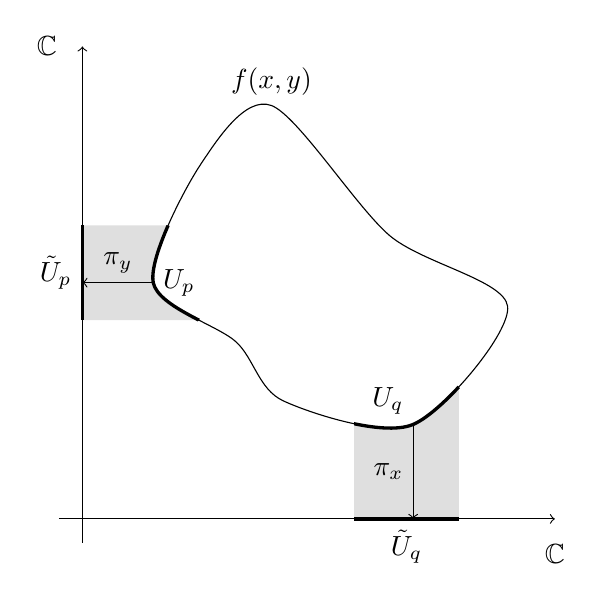
\begin{tikzpicture}[scale=1.5]
	\coordinate (x) at (4,0);
	\coordinate (y) at (0,4);
	\draw[->] (-0.2,0) to (x) node[below=0.2cm]{$ \mathbb{C} $};
	\draw[->] (0,-0.2) to (y) node[left=0.2cm]{$ \mathbb{C} $};

	\coordinate (a) at (0.6,2);
	\coordinate (b) at (2.8,0.8);
	\coordinate (l) at (1.6,3.5);

	\begin{scope}
		\clip[name path global=ac] (a) circle (0.5);
		\curve[name path global=ap];
	\end{scope}
	\fill[fill=gray!50, fill opacity=0.5, name intersections={of=ac and ap}]
	(intersection-1) -- (intersection-2) -- ($ (0,0)!(intersection-2)!(y) $) -- ($
	(0,0)!(intersection-1)!(y) $) -- cycle;
	\draw[very thick, name intersections={of=ac and ap}] ($
	(0,0)!(intersection-1)!(y) $) to node[left]{$ \tilde{U} _{p} $} ($
	(0,0)!(intersection-2)!(y) $);

	\begin{scope}
		\clip[name path global=bc] (b) circle (0.5);
		\curve[name path global=bp];
	\end{scope}
	\fill[fill=gray!50, fill opacity=0.5, name intersections={of=bc and bp}]
	(intersection-1) -- (intersection-2) -- ($ (0,0)!(intersection-2)!(x) $) -- ($
	(0,0)!(intersection-1)!(x) $) -- cycle;
	\draw[very thick, name intersections={of=bc and bp}] ($
	(0,0)!(intersection-1)!(x) $) to node[below]{$ \tilde{U} _{q} $} ($
	(0,0)!(intersection-2)!(x) $);

	\curve[fill=white];
	\begin{scope}
		\clip (b) circle (0.5);
		\curve[very thick];
	\end{scope}
	\begin{scope}
		\clip (a) circle (0.5);
		\curve[very thick];
	\end{scope}

	\node[right] at (a){$ U _{p} $};
	\node[above left] at (b){$ U _{q} $};
	\node[above] at (l){$ f(x,y) $};

	\draw[->] (a) to node[above]{$ \pi_y $} ($ (0,0)!(a)!(y) $);
	\draw[->] (b) to node[left]{$ \pi_x $} ($ (0,0)!(b)!(x) $);


\end{tikzpicture}
\end{document}
